\title[Case studies]{Case studies and teardown session}
\section{Case studies}

\begin{frame}[plain]
	\titlepage
\end{frame}

%%%%%%%%%%%%%%%%%%%%%%%%%%%%%%%%%%%%%%%%%%%%%%%%%%%%%%%%%%%%%
%% Format %%
%%%%%%%%%%%%%%%%%%%%%%%%%%%%%%%%%%%%%%%%%%%%%%%%%%%%%%%%%%%%%
\subsection{Format}

\begin{frame}
	\frametitle{Format of the session}
	\begin{columns}[T]
		\begin{column}{0.5\textwidth}
			\begin{table}
				\centering
				\footnotesize
				\begin{tabular}{|l|>{\raggedright\arraybackslash}p{4.4cm}|}
					\hline
					20\,min & guided walkthrough of five cases                              \\
					50\,min & stations A to E, teams of three or four, 10\,min per station \\
					20\,min & synthesis, quiz and design duel                               \\
					\hline
				\end{tabular}
				\caption{Timetable}
			\end{table}
			\small
			\textbf{Rules}
			\begin{itemize}
				\item Mains-powered products are examined unpowered only. Do not reconnect them.
				\item Bulk capacitors may still be charged: measure before touching.
				\item Open boards: ESD wrist strap.
			\end{itemize}
		\end{column}
		\begin{column}{0.46\textwidth}
			\small
			\textbf{At every station}
			\begin{enumerate}
				\item Follow the power path from input to output.
				\item Identify switches, magnetics and capacitors; read the part numbers.
				\item Find the commutation loop and estimate its inductance (L3).
				\item Estimate $f_\mathrm{sw}$ from the components.
				\item Sketch the loss budget: the three largest losses.
			\end{enumerate}
			Record everything on the worksheet of the station; it is part of your design portfolio.
		\end{column}
	\end{columns}
\end{frame}

%%%%%%%%%%%%%%%%%%%%%%%%%%%%%%%%%%%%%%%%%%%%%%%%%%%%%%%%%%%%%
%% Case A %%
%%%%%%%%%%%%%%%%%%%%%%%%%%%%%%%%%%%%%%%%%%%%%%%%%%%%%%%%%%%%%
\subsection{Case A: GaN charger}

\begin{frame}
	\frametitle{Case A: GaN USB-C charger}
	\begin{figure}
		\centering
		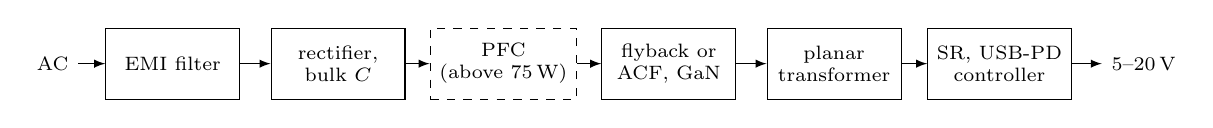
\begin{tikzpicture}[font=\scriptsize, >=latex, box/.style={draw, minimum width=1.7cm, minimum height=0.9cm, align=center}]
			\node[box] (emi) at (0,0) {EMI filter};
			\node[box] (rec) at (2.1,0) {rectifier,\\bulk $C$};
			\node[box, dashed] (pfc) at (4.2,0) {PFC\\(above 75\,W)};
			\node[box] (fly) at (6.3,0) {flyback or\\ACF, GaN};
			\node[box] (tr) at (8.4,0) {planar\\transformer};
			\node[box] (sr) at (10.5,0) {SR, USB-PD\\controller};
			\draw[->] (-1.2,0) node[left]{AC} -- (emi);
			\draw[->] (emi) -- (rec); \draw[->] (rec) -- (pfc); \draw[->] (pfc) -- (fly); \draw[->] (fly) -- (tr); \draw[->] (tr) -- (sr);
			\draw[->] (sr) -- (11.8,0) node[right]{5--20\,V};
		\end{tikzpicture}
		\caption{Power path of a USB-C charger. Dashed: only above 75\,W; ACF: active-clamp flyback; SR: synchronous rectifier}
	\end{figure}
	\vspace{-0.2cm}
	\footnotesize
	\begin{itemize}
		\item Up to 75\,W input power IEC 61000-3-2 sets no harmonic limits for such equipment: no PFC stage. Above 75\,W a boost PFC stage is added.
		\item Primary: quasi-resonant flyback with valley switching, or active-clamp flyback with ZVS through the clamp (L8); GaN power ICs with integrated driver (L4).
		\item Planar or RM-core transformer with interleaved windings (L7); a synchronous rectifier replaces the secondary diode.
		\item A Y-capacitor across the isolation barrier returns the common-mode current to the primary; the permitted touch current limits its value (L14).
		\item USB Power Delivery (PD): fixed voltages 5, 9, 15 and 20\,V, up to 100\,W; PD 3.1 extends to 48\,V and 240\,W.
	\end{itemize}
	\blfootnote{Sources: L8 (active-clamp flyback controllers and reference designs); IEC 61000-3-2; USB Power Delivery specification, USB-IF.}
\end{frame}

%%%%%%%%%%%%%%%%%%%%%%%%%%%%%%%%%%%%%%%%%%%%%%%%%%%%%%%%%%%%%
%% Charger: what shrinks %%
%%%%%%%%%%%%%%%%%%%%%%%%%%%%%%%%%%%%%%%%%%%%%%%%%%%%%%%%%%%%%
\begin{frame}
	\frametitle{What does not shrink}
	\begin{columns}[T]
		\begin{column}{0.5\textwidth}
			\footnotesize
			The bulk capacitor alone supplies the input power $P_\mathrm{in}$ for the time $t_\mathrm{d}$ of each half cycle and must not fall below $V_\mathrm{min}$ ($V_\mathrm{pk}$: peak line voltage):
			\begin{equation*}
				C\geq\frac{2P_\mathrm{in}t_\mathrm{d}}{V_\mathrm{pk}^2-V_\mathrm{min}^2}
			\end{equation*}
			65\,W, $\eta=92$\,\%, 90\,V AC at 50\,Hz: $V_\mathrm{pk}=127$\,V. For $V_\mathrm{min}=80$\,V the line recharges the capacitor from $39^\circ$ to $90^\circ$ of each half cycle; the rest is $t_\mathrm{d}=7.2$\,ms:
			\begin{equation*}
				C\geq\frac{2\cdot70.7\,\mathrm{W}\cdot7.2\,\mathrm{ms}}{(127\,\mathrm{V})^2-(80\,\mathrm{V})^2}=104\,\mu\mathrm{F},\ 400\,\mathrm{V}
			\end{equation*}
			The 400\,V rating covers 264\,V AC. The value does not depend on $f_\mathrm{sw}$: energy storage at line frequency.
		\end{column}
		\begin{column}{0.47\textwidth}
			\footnotesize
			\textbf{Shrinks with $f_\mathrm{sw}$}: transformer (volt-seconds per turn), output filter, the switching-frequency part of the EMI filter.
			\vspace{0.2cm}

			\textbf{Does not shrink}: bulk capacitor, safety distances (creepage and clearance), connector, the low-frequency end of the EMI filter at 150\,kHz.
			\vspace{0.2cm}

			With $f_\mathrm{sw}$ below 150\,kHz the switching fundamental lies outside the conducted-emission band (150\,kHz to 30\,MHz); above 150\,kHz the filter must also attenuate the fundamental (L14).
			\vspace{0.2cm}

			Example: 65\,W in a case of $45\times45\times30$\,mm$^3$: 1.07\,W/cm$^3$ (17.5\,W/in$^3$), counted on the outer volume of the case.
		\end{column}
	\end{columns}
	\blfootnote{L1: scaling of passive components; CISPR 32 (conducted emissions from 150\,kHz).}
\end{frame}

%%%%%%%%%%%%%%%%%%%%%%%%%%%%%%%%%%%%%%%%%%%%%%%%%%%%%%%%%%%%%
%% Case B %%
%%%%%%%%%%%%%%%%%%%%%%%%%%%%%%%%%%%%%%%%%%%%%%%%%%%%%%%%%%%%%
\subsection{Case B: bus converter}

\begin{frame}
	\frametitle{Case B: 48\,V bus converter}
	\begin{figure}
		\centering
		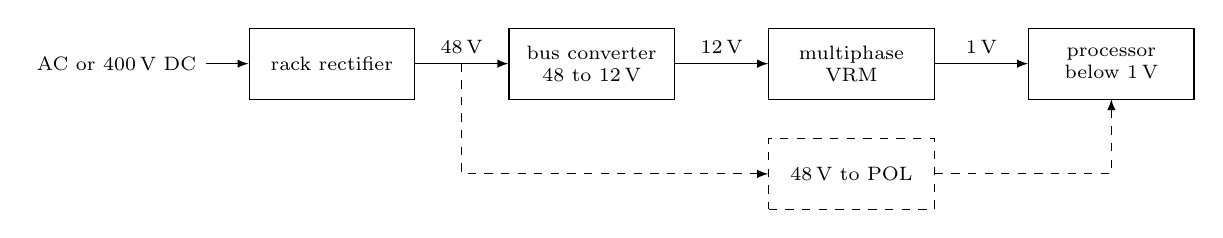
\begin{tikzpicture}[font=\scriptsize, >=latex, box/.style={draw, minimum width=2.1cm, minimum height=0.9cm, align=center}]
			\node[box] (psu) at (0,0) {rack rectifier};
			\node[box] (bus) at (3.3,0) {bus converter\\48 to 12\,V};
			\node[box] (vrm) at (6.6,0) {multiphase\\VRM};
			\node[box] (cpu) at (9.9,0) {processor\\below 1\,V};
			\node[box, dashed] (pol) at (6.6,-1.4) {48\,V to POL};
			\draw[->] (-1.6,0) node[left]{AC or 400\,V DC} -- (psu);
			\draw[->] (psu) -- node[above]{48\,V} (bus);
			\draw[->] (bus) -- node[above]{12\,V} (vrm);
			\draw[->] (vrm) -- node[above]{1\,V} (cpu);
			\draw[->, dashed] (1.65,0) |- (pol.west);
			\draw[->, dashed] (pol.east) -| (9.9,-0.45);
		\end{tikzpicture}
		\caption{Power delivery in a data centre: intermediate bus (solid) or direct 48\,V to point of load (dashed)}
	\end{figure}
	\vspace{-0.2cm}
	\footnotesize
	\begin{itemize}
		\item 48\,V instead of 12\,V on the rack: a quarter of the current and $1/16$ of the $I^2R$ loss in the same conductors.
		\item The chain efficiency is the product of all stages: three stages of 97\,\% give 91\,\%.
		\item The bus converter needs no regulation, since the VRM after it regulates: an LLC at $f_\mathrm{r}$ with a fixed ratio (DCX, L9), a matrix transformer (L7) and synchronous rectifiers. Research example: 380 to 12\,V, 1\,kW, 1\,MHz, above 97\,\%.
	\end{itemize}
	\blfootnote{Sources: Y. Zhu et al., in Kizilyalli et al.\ (eds.), \textit{Wide Bandgap Power Electronics}, Springer, 2025, ch.\ 18; Ranjram and Perreault, 2022; Perreault, APEC 2024 plenary.}
\end{frame}

%%%%%%%%%%%%%%%%%%%%%%%%%%%%%%%%%%%%%%%%%%%%%%%%%%%%%%%%%%%%%
%% Reading a DCX %%
%%%%%%%%%%%%%%%%%%%%%%%%%%%%%%%%%%%%%%%%%%%%%%%%%%%%%%%%%%%%%
\begin{frame}
	\frametitle{Reading a DCX}
	\begin{columns}[T]
		\begin{column}{0.5\textwidth}
			\footnotesize
			\begin{itemize}
				\item Ratio from the label or the turns: 48 to 12\,V, $n=4$.
				\item Resonant capacitors: number times value gives $C_\mathrm{r}$. A DCX switches at its resonant frequency, so $f_\mathrm{sw}$ from the controller gives the tank inductance:
				\begin{equation*}
					L_\mathrm{r}=\frac{1}{(2\pi f_\mathrm{sw})^2C_\mathrm{r}}
				\end{equation*}
				685\,nF at 1\,MHz: 37\,nH, the leakage inductance of the B2 design in L9.
				\item Magnetising inductance from the air gap or the core data: is $L_\mathrm{m}$ small enough that its current completes the ZVS transition within the dead time (L9)?
			\end{itemize}
		\end{column}
		\begin{column}{0.47\textwidth}
			\footnotesize
			\begin{itemize}
				\item Synchronous rectifiers (SR): count and $R_\mathrm{DS(on)}$; their conduction loss $I_\mathrm{rms}^2R_\mathrm{DS(on)}$ at full load is often the largest single loss.
				\item Heat path: where do transformer and SRs dissipate, and through which pad or heat sink (L14)?
				\item Power density from the outer dimensions, without and with heat sink.
			\end{itemize}
			\begin{block}{Key message}
				A DCX is read from its capacitors and its transformer: $C_\mathrm{r}$ and $f_\mathrm{sw}$ fix $L_\mathrm{r}$.
			\end{block}
		\end{column}
	\end{columns}
\end{frame}

%%%%%%%%%%%%%%%%%%%%%%%%%%%%%%%%%%%%%%%%%%%%%%%%%%%%%%%%%%%%%
%% Case C %%
%%%%%%%%%%%%%%%%%%%%%%%%%%%%%%%%%%%%%%%%%%%%%%%%%%%%%%%%%%%%%
\subsection{Case C: VRM and integration}

\begin{frame}
	\frametitle{Case C: VRM and integration}
	\begin{columns}[T]
		\begin{column}{0.52\textwidth}
			\begin{table}
				\centering
				\scriptsize
				\begin{tabular}{|l|>{\raggedright\arraybackslash}p{2.0cm}|>{\raggedright\arraybackslash}p{2.3cm}|}
					\hline
					                   & \textbf{FIVR}                    & \textbf{Mini-LEGO}                                     \\
					\hline
					conversion         & 1.8\,V to about 1\,V             & 48\,V to 1\,V, 240\,A                                  \\
					topology           & multiphase buck, up to 16 phases per domain & 3 stacked 2:1 SC units, 12 buck phases       \\
					$f_\mathrm{sw}$    & 140\,MHz                         & SC 433\,kHz, buck 1.5\,MHz                             \\
					inductors          & air core in the package layers   & vertical coupled inductors, 2.5\,mm                    \\
					efficiency         & about 90\,\% peak                & 87.1\,\% peak, 84.1\,\% at 240\,A                      \\
					density            & 31\,A/mm$^2$                     & 0.71\,A/mm$^2$, 1390\,W/in$^3$                         \\
					\hline
				\end{tabular}
				\caption{Integrated regulator and 48\,V module; density: current per board area}
			\end{table}
		\end{column}
		\begin{column}{0.45\textwidth}
			\footnotesize
			\begin{itemize}
				\item The closer to the load, the lower the voltage and the higher the frequency.
				\item FIVR (fully integrated voltage regulator, Intel) puts the last stage into the processor package: 8 to 31 separately supplied voltage domains, each rail ramps in about 0.5\,$\mu$s.
				\item Mini-LEGO (48\,V to 1\,V research module): the switched-capacitor (SC) stage divides 48\,V to an 8\,V intermediate bus. The buck inductors carry the charging current of the flying capacitors, so they charge without current spikes (soft charging). Only 8.4\,mm high: it fits under the processor (vertical power delivery).
			\end{itemize}
		\end{column}
	\end{columns}
	\blfootnote{Sources: E.\,A. Burton et al., IEEE APEC 2014, pp.\ 432--439; Y. Elasser et al., IEEE APEC 2023.}
\end{frame}

%%%%%%%%%%%%%%%%%%%%%%%%%%%%%%%%%%%%%%%%%%%%%%%%%%%%%%%%%%%%%
%% Interleaving %%
%%%%%%%%%%%%%%%%%%%%%%%%%%%%%%%%%%%%%%%%%%%%%%%%%%%%%%%%%%%%%
\begin{frame}
	\frametitle{Interleaving at low duty cycle}
	\begin{columns}[T]
		\begin{column}{0.5\textwidth}
			\begin{figure}
				\centering
				\begin{tikzpicture}
					\begin{axis}[
							width=\linewidth, height=4.8cm,
							xmin=0, xmax=1, ymin=0, ymax=1.25, ytick={0,0.25,0.5,0.75,1},
							xlabel={$D$}, ylabel={$\Delta i_\mathrm{sum}/\Delta i_\mathrm{phase}$},
							grid=major, grid style={gray!20},
							tick label style={font=\scriptsize}, label style={font=\footnotesize},
							legend style={font=\tiny, at={(0.5,0.97)}, anchor=north}, legend columns=3,
						]
						\addplot[black, thick] table[x=D, y=K2] {fig/lec11/interleave.dat};
						\addlegendentry{$N=2$}
						\addplot[black, thick, dashed] table[x=D, y=K3] {fig/lec11/interleave.dat};
						\addlegendentry{$N=3$}
						\addplot[black, thick, dotted] table[x=D, y=K4] {fig/lec11/interleave.dat};
						\addlegendentry{$N=4$}
					\end{axis}
				\end{tikzpicture}
				\caption{Ripple of the summed current of $N$ interleaved phases, relative to the ripple of one phase}
			\end{figure}
		\end{column}
		\begin{column}{0.47\textwidth}
			\footnotesize
			With $m=\lfloor ND\rfloor$, the largest integer not above $ND$:
			\begin{equation*}
				\frac{\Delta i_\mathrm{sum}}{\Delta i_\mathrm{phase}}=\frac{N\left(D-\frac{m}{N}\right)\left(\frac{m+1}{N}-D\right)}{D(1-D)}
			\end{equation*}
			\begin{itemize}
				\item The ripple cancels completely at $D=k/N$ ($k$ integer); the summed current ripples at $Nf_\mathrm{sw}$.
				\item For $D<1/N$ the factor is $(1-ND)/(1-D)$: at 12 to 1\,V ($D=0.083$) four phases still leave 73\,\% of the ripple of one phase.
				\item Low duty cycle needs many phases, coupled inductors (L7) or an intermediate step such as the 8\,V bus of the Mini-LEGO.
			\end{itemize}
		\end{column}
	\end{columns}
	\blfootnote{Computed with \texttt{interleave.py} (numerical check of the formula).}
\end{frame}

%%%%%%%%%%%%%%%%%%%%%%%%%%%%%%%%%%%%%%%%%%%%%%%%%%%%%%%%%%%%%
%% Case D %%
%%%%%%%%%%%%%%%%%%%%%%%%%%%%%%%%%%%%%%%%%%%%%%%%%%%%%%%%%%%%%
\subsection{Case D: wireless power}

\begin{frame}
	\frametitle{Case D: 6.78\,MHz transmitter}
	\begin{figure}
		\centering
		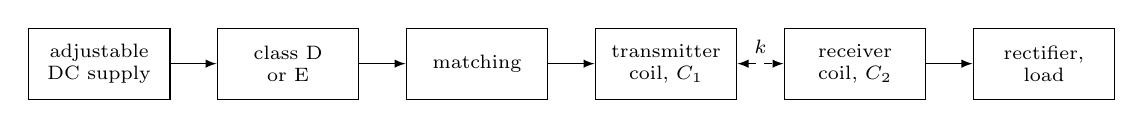
\begin{tikzpicture}[font=\scriptsize, >=latex, box/.style={draw, minimum width=1.8cm, minimum height=0.9cm, align=center}]
			\node[box] (dc) at (0,0) {adjustable\\DC supply};
			\node[box] (inv) at (2.4,0) {class D\\or E};
			\node[box] (mn) at (4.8,0) {matching};
			\node[box] (tx) at (7.2,0) {transmitter\\coil, $C_1$};
			\node[box] (rx) at (9.6,0) {receiver\\coil, $C_2$};
			\node[box] (rc) at (12.0,0) {rectifier,\\load};
			\draw[->] (dc) -- (inv); \draw[->] (inv) -- (mn); \draw[->] (mn) -- (tx);
			\draw[<->, dashed] (tx) -- node[above]{$k$} (rx); \draw[->] (rx) -- (rc);
		\end{tikzpicture}
		\caption{Transmitter and receiver of an inductive link; $k$: coupling factor of the two coils}
	\end{figure}
	\vspace{-0.2cm}
	\small
	\begin{itemize}
		\item Tutorial 10, brief B4: for $k=0.10$ to 0.25 the resistance seen at the primary changes from 2.4 to 13.8\,$\Omega$. A class E with fixed tuning and supply then delivers 5 to 27\,W, and its switch voltage reaches 101\,V.
		\item The power is therefore controlled by the DC supply voltage of the inverter (14 to 33\,V for a class D half-bridge) or on the receiver side.
		\item Coil $Q$ of a few hundred; a ferrite sheet behind the coil guides the flux and shields the electronics.
		\item The AirFuel Resonant standard uses the 6.78\,MHz ISM band (IEC 63028:2017).
	\end{itemize}
\end{frame}

%%%%%%%%%%%%%%%%%%%%%%%%%%%%%%%%%%%%%%%%%%%%%%%%%%%%%%%%%%%%%
%% Reading a transmitter %%
%%%%%%%%%%%%%%%%%%%%%%%%%%%%%%%%%%%%%%%%%%%%%%%%%%%%%%%%%%%%%
\begin{frame}
	\frametitle{Reading a transmitter}
	\begin{columns}[T]
		\begin{column}{0.5\textwidth}
			\small
			\begin{itemize}
				\item Coil: turns and diameter; inductance with the LCR meter at 1\,MHz. At 6.78\,MHz the self-resonance raises the apparent inductance: measure it with the impedance analyser (L5).
				\item Tuning capacitors: $f_\mathrm{r}=1/(2\pi\sqrt{L_1C_1})$ should lie at 6.78\,MHz; 1.2\,$\mu$H needs 459\,pF.
				\item Count the switches: class D (two, high-side driver) or class E (one, choke).
			\end{itemize}
		\end{column}
		\begin{column}{0.47\textwidth}
			\small
			\begin{itemize}
				\item Find the matching network: which elements are C0G, which inductors air core?
				\item How is the power controlled: a buck or buck-boost stage in front of the inverter?
				\item Where are the shields and the ferrite sheet? Which path does the common-mode current take?
			\end{itemize}
			\begin{block}{Key message}
				A WPT transmitter is a resonant inverter whose load moves with the receiver.
			\end{block}
		\end{column}
	\end{columns}
\end{frame}

%%%%%%%%%%%%%%%%%%%%%%%%%%%%%%%%%%%%%%%%%%%%%%%%%%%%%%%%%%%%%
%% Case E %%
%%%%%%%%%%%%%%%%%%%%%%%%%%%%%%%%%%%%%%%%%%%%%%%%%%%%%%%%%%%%%
\subsection{Case E: IAS CLLC model}

\begin{frame}
	\frametitle{Case E: IAS 11\,kW CLLC model}
	\begin{table}
		\centering
		\scriptsize
		\begin{tabular}{|l|c|c|>{\raggedright\arraybackslash}p{5.3cm}|}
			\hline
			                                  & \textbf{125\,kHz}   & \textbf{1\,MHz}        & \textbf{Consequence}                                              \\
			\hline
			primary tank at the same $Z_0$    & 30\,$\mu$H, 181\,nF & 3.75\,$\mu$H, 22.6\,nF & eight times smaller; leakage and wiring become a large part        \\
			ZVS current, dead time 2.5\,\% of $T$ & 0.9\,A           & 7.1\,A                 & eight times the current; with 0.9\,A the dead time would be 20\,\% of $T$ \\
			copper skin depth at 100\,$^\circ$C & 214\,$\mu$m       & 76\,$\mu$m             & litz strands three times thinner                                   \\
			gate-drive power                  & $P_\mathrm{G}$      & $8P_\mathrm{G}$        & $Q_\mathrm{G}V_\mathrm{GS}f$: driver dissipation and supply rise accordingly (L4) \\
			volt-seconds per half period      & 1                   & 1/8                    & fewer turns or less core area, but a higher core-loss density (L6) \\
			\hline
		\end{tabular}
		\caption{IAS CLLC simulation model (11\,kW, 700 to 845\,V, SiC, about 40\,m$\Omega$) scaled from 125\,kHz to 1\,MHz at the same $Z_0$ and $f_\mathrm{sw}/f_\mathrm{r}$; $T$: period}
	\end{table}
	\vspace{-0.4cm}
	\footnotesize
	\begin{itemize}
		\item Devices: the $C_\mathrm{oss}$ hysteresis loss of SiC rises with $f$ (L2); 1200\,V GaN is not established at this power (L9).
		\item EMI: the fundamental moves into the conducted-emission band, which starts at 150\,kHz; a filter for 1\,MHz is smaller, though (L14).
		\item Hardware at IAS: TI reference design PMP41042, a 3.6\,kW CLLLC (380--410\,V to 40--60\,V, about 170\,kHz).
	\end{itemize}
	\blfootnote{Sources: IAS LTspice simulation model \texttt{CLLC\_sim\_new\_resonant\_tank\_11kW}, scaled as in L9; TI PMP41042 and test report TIDT367, 2023.}
\end{frame}

%%%%%%%%%%%%%%%%%%%%%%%%%%%%%%%%%%%%%%%%%%%%%%%%%%%%%%%%%%%%%
%% Paths to MHz %%
%%%%%%%%%%%%%%%%%%%%%%%%%%%%%%%%%%%%%%%%%%%%%%%%%%%%%%%%%%%%%
\begin{frame}
	\frametitle{Paths to 1\,MHz at 11\,kW}
	\begin{columns}[T]
		\begin{column}{0.48\textwidth}
			\small
			\textbf{Options to judge}
			\begin{enumerate}[(a)]
				\item One converter with SiC at 1\,MHz and a planar matrix transformer.
				\item Modules in input-series, output-parallel connection: lower voltage per module, 650\,V GaN.
				\item A flying-capacitor or stacked bridge: half the voltage per switch.
				\item Stay at 125 to 300\,kHz and optimise the magnetics.
			\end{enumerate}
		\end{column}
		\begin{column}{0.48\textwidth}
			\small
			\textbf{Criteria}
			\begin{itemize}
				\item ZVS charge within the dead time at the worst-case operating point.
				\item Loss per device including $C_\mathrm{oss}$ hysteresis and gate drive.
				\item Transformer loss with the optimum flux density, and the winding at the new skin depth.
				\item Insulation and creepage at 845\,V, cooling, EMI.
			\end{itemize}
		\end{column}
	\end{columns}
	\begin{block}{Key message}
		At 11\,kW the frequency is limited by the devices and the transformer together; MHz operation needs a different architecture, not a scaled tank.
	\end{block}
\end{frame}

%%%%%%%%%%%%%%%%%%%%%%%%%%%%%%%%%%%%%%%%%%%%%%%%%%%%%%%%%%%%%
%% Synthesis %%
%%%%%%%%%%%%%%%%%%%%%%%%%%%%%%%%%%%%%%%%%%%%%%%%%%%%%%%%%%%%%
\subsection{Synthesis}

\begin{frame}
	\frametitle{Common patterns}
	\begin{columns}[T]
		\begin{column}{0.48\textwidth}
			\small
			\textbf{Seen in all five cases}
			\begin{itemize}
				\item Soft switching everywhere: by the magnetising current (DCX), the clamp of the active-clamp flyback, the tank (class D/E) or the inductor current (VRM).
				\item The frequency rises towards the load: about 100\,kHz to 1\,MHz in AC-DC and bus converters, 1.5\,MHz in the 48\,V module, 140\,MHz in the package.
				\item Energy storage at line frequency (bulk capacitor) does not shrink with $f_\mathrm{sw}$.
				\item The magnetics decide the size: planar, matrix, coupled or air-core designs.
			\end{itemize}
		\end{column}
		\begin{column}{0.48\textwidth}
			\small
			\textbf{Open problems}
			\begin{itemize}
				\item Magnetic materials above 10\,MHz.
				\item $C_\mathrm{oss}$ losses of GaN and SiC at MHz frequencies.
				\item EMI and heat removal of dense designs.
				\item Regulation of resonant stages over wide ranges.
			\end{itemize}
			\vspace{0.2cm}
			Optional holiday challenge: efficiency versus power density (Pareto front) of the buck in triangular current mode (TCM) of Tutorial 8, with the course notebooks.
		\end{column}
	\end{columns}
	\blfootnote{Source: Perreault, APEC 2024 plenary (open problems of high-frequency power conversion).}
\end{frame}

%%%%%%%%%%%%%%%%%%%%%%%%%%%%%%%%%%%%%%%%%%%%%%%%%%%%%%%%%%%%%
%% Station worksheets %%
%%%%%%%%%%%%%%%%%%%%%%%%%%%%%%%%%%%%%%%%%%%%%%%%%%%%%%%%%%%%%
\subsection{Stations}

\begin{frame}
	\frametitle{Station A: charger}
	\footnotesize
	\renewcommand{\arraystretch}{1.5}
	\begin{tabular}{|>{\raggedright\arraybackslash}p{6.2cm}|p{6.6cm}|l|}
		\hline
		\textbf{Task}                                                                  & \textbf{Finding} & \textbf{Ref.} \\
		\hline
		Input stage: fuse, X and Y capacitors, common-mode choke                       &                  & L14           \\
		PFC stage present? Rating against 75\,W                                        &                  & L11           \\
		Primary topology: number of switches, clamp capacitor, controller part number  &                  & L8            \\
		$f_\mathrm{sw}$ from the controller data sheet and its setting components      &                  & L8            \\
		Transformer: core type and size, $A_\mathrm{e}$ from the core data             &                  & L6, L7        \\
		Primary loop: area, spacing, estimated inductance                              &                  & L3            \\
		Bulk capacitor: value against 104\,$\mu$F for 65\,W at 90\,V AC                 &                  & L11           \\
		\hline
	\end{tabular}
\end{frame}

\begin{frame}
	\frametitle{Station B: bus converter}
	\footnotesize
	\renewcommand{\arraystretch}{1.5}
	\begin{tabular}{|>{\raggedright\arraybackslash}p{6.2cm}|p{6.6cm}|l|}
		\hline
		\textbf{Task}                                                                  & \textbf{Finding} & \textbf{Ref.} \\
		\hline
		Ratio and topology: bridges on both sides, transformer structure               &                  & L7, L9        \\
		Resonant capacitors: number, value, dielectric; total $C_\mathrm{r}$           &                  & L9, L10       \\
		$f_\mathrm{sw}$ and the resulting $L_\mathrm{r}=1/((2\pi f_\mathrm{sw})^2C_\mathrm{r})$ &         & L9            \\
		Synchronous rectifiers: number, $R_\mathrm{DS(on)}$, conduction loss at full load &               & L9            \\
		Heat path of transformer and rectifiers                                        &                  & L14           \\
		Power density with and without heat sink                                       &                  & L1            \\
		\hline
	\end{tabular}
\end{frame}

\begin{frame}
	\frametitle{Station C: voltage regulator}
	\footnotesize
	\renewcommand{\arraystretch}{1.5}
	\begin{tabular}{|>{\raggedright\arraybackslash}p{6.2cm}|p{6.6cm}|l|}
		\hline
		\textbf{Task}                                                                  & \textbf{Finding} & \textbf{Ref.} \\
		\hline
		Number of phases, power stages (part numbers), controller                      &                  & L4            \\
		Inductors: value, size, coupled or not                                         &                  & L7            \\
		$f_\mathrm{sw}$ from the ripple $\Delta i=V_\mathrm{o}(1-D)/(Lf_\mathrm{sw})$ or the data sheet &   & L8            \\
		Ripple cancellation at the operating duty cycle (previous slide)              &                  & L11           \\
		Output capacitors: number, type, placement under the load                      &                  & L3, L13       \\
		Input loop of each phase: area and estimated inductance                       &                  & L3            \\
		\hline
	\end{tabular}
\end{frame}

\begin{frame}
	\frametitle{Station D: wireless power}
	\footnotesize
	\renewcommand{\arraystretch}{1.5}
	\begin{tabular}{|>{\raggedright\arraybackslash}p{6.2cm}|p{6.6cm}|l|}
		\hline
		\textbf{Task}                                                                  & \textbf{Finding} & \textbf{Ref.} \\
		\hline
		Coil: turns, diameter, inductance at 1\,MHz, ferrite sheet                     &                  & L7, L10       \\
		Tuning capacitors and $f_\mathrm{r}$                                           &                  & L10           \\
		Inverter: class D or E, switches, gate drive                                   &                  & L4, L10       \\
		Matching network: elements and their technology                                &                  & L10           \\
		Power control: stage in front of the inverter?                                 &                  & L10           \\
		Shielding and common-mode path                                                 &                  & L14           \\
		\hline
	\end{tabular}
\end{frame}

\begin{frame}
	\frametitle{Station E: IAS CLLC model}
	\footnotesize
	\renewcommand{\arraystretch}{1.5}
	\begin{tabular}{|>{\raggedright\arraybackslash}p{6.2cm}|p{6.6cm}|l|}
		\hline
		\textbf{Task (laptop with the IAS LTspice simulation model)}                   & \textbf{Finding} & \textbf{Ref.} \\
		\hline
		Run the model at 11\,kW: switch currents at the switching instants             &                  & L8, L9        \\
		Charge needed for ZVS and the available dead time                              &                  & L8            \\
		Scale the tank to 1\,MHz and run again: what fails first?                      &                  & L9            \\
		Estimate device and gate losses at 125\,kHz and 1\,MHz                         &                  & L2, L4        \\
		Choose one of the paths (a) to (d) and justify it with two numbers             &                  & L11           \\
		\hline
	\end{tabular}
	\vspace{0.2cm}

	The 11\,kW CLLC exists as a simulation model; hardware tests at IAS use the TI reference design PMP41042 (3.6\,kW CLLLC, 380--410\,V to 40--60\,V).
\end{frame}

%%%%%%%%%%%%%%%%%%%%%%%%%%%%%%%%%%%%%%%%%%%%%%%%%%%%%%%%%%%%%
%% Quiz %%
%%%%%%%%%%%%%%%%%%%%%%%%%%%%%%%%%%%%%%%%%%%%%%%%%%%%%%%%%%%%%
\subsection{Quiz and design duel}

% Two pages: question (page 1) and answer (page 2).
\begin{frame}<handout:1-2>
	\frametitle{Quiz 1: the bulk capacitor}
	\begin{columns}[T]
		\begin{column}{0.48\textwidth}
			\small
			A 65\,W charger moves from 100\,kHz to 1\,MHz. Which component keeps its size?
			\begin{enumerate}[A]
				\item the transformer
				\item the output capacitor
				\item the bulk capacitor
				\item the differential-mode inductor of the EMI filter
			\end{enumerate}
		\end{column}
		\begin{column}{0.48\textwidth}
			\onslide<2-|handout:2>{
				\begin{block}{Answer: C}
					The bulk capacitor bridges the line-frequency valleys (104\,$\mu$F for 65\,W at 90\,V AC). Transformer and output capacitor shrink with $f_\mathrm{sw}$; the EMI filter shrinks partly, since the limits start at 150\,kHz.
				\end{block}
			}
		\end{column}
	\end{columns}
\end{frame}

% Two pages: question (page 1) and answer (page 2).
\begin{frame}<handout:1-2>
	\frametitle{Quiz 2: the rack voltage}
	\begin{columns}[T]
		\begin{column}{0.48\textwidth}
			\small
			A rack bus changes from 12\,V to 48\,V at the same power and with the same conductors. The distribution loss becomes
			\begin{enumerate}[A]
				\item one half
				\item one quarter
				\item one sixteenth
				\item unchanged, since the power is the same
			\end{enumerate}
		\end{column}
		\begin{column}{0.48\textwidth}
			\onslide<2-|handout:2>{
				\begin{block}{Answer: C}
					The current falls by four, the $I^2R$ loss by sixteen. The price is a converter with a larger step-down ratio near the load (Case C).
				\end{block}
			}
		\end{column}
	\end{columns}
\end{frame}

% Two pages: question (page 1) and answer (page 2).
\begin{frame}<handout:1-2>
	\frametitle{Quiz 3: inductors at 140\,MHz}
	\begin{columns}[T]
		\begin{column}{0.48\textwidth}
			\small
			Which inductors does FIVR use at 140\,MHz?
			\begin{enumerate}[A]
				\item ferrite chip inductors on the motherboard
				\item air-core inductors in the metal layers of the package
				\item coupled inductors with powder cores
				\item no inductors: it is a switched-capacitor converter
			\end{enumerate}
		\end{column}
		\begin{column}{0.48\textwidth}
			\onslide<2-|handout:2>{
				\begin{block}{Answer: B}
					At 140\,MHz small air-core inductors in the package suffice and no core loss arises; the output capacitance sits on the die. The input is about 1.8\,V from a first-stage regulator on the board.
				\end{block}
			}
		\end{column}
	\end{columns}
\end{frame}

%%%%%%%%%%%%%%%%%%%%%%%%%%%%%%%%%%%%%%%%%%%%%%%%%%%%%%%%%%%%%
%% Design duel %%
%%%%%%%%%%%%%%%%%%%%%%%%%%%%%%%%%%%%%%%%%%%%%%%%%%%%%%%%%%%%%
\begin{frame}
	\frametitle{Design duel}
	\begin{columns}[T]
		\begin{column}{0.48\textwidth}
			\small
			\textbf{Rules}
			\begin{itemize}
				\item Each team defends the topology of its brief in two minutes: topology, $f_\mathrm{sw}$, the critical component, the largest risk.
				\item One question from another team, one minute to answer.
				\item Numbers, not adjectives: every claim with a value and the lecture it comes from.
			\end{itemize}
		\end{column}
		\begin{column}{0.48\textwidth}
			\small
			\textbf{Peers judge}
			\begin{itemize}
				\item Is the soft-switching condition checked at the worst case?
				\item Is the loss budget complete (devices, magnetics, gate, capacitors)?
				\item Does the frequency follow from the design, or was it chosen first?
				\item Is the risk named together with the test that removes it?
			\end{itemize}
		\end{column}
	\end{columns}
\end{frame}

\begin{frame}
	\frametitle{Layout clinic}
	\begin{columns}[T]
		\begin{column}{0.48\textwidth}
			\small
			Bring your current layout; we check it in the last 20 minutes.
			\begin{enumerate}
				\item Commutation loop: area, return path in the adjacent layer (L3).
				\item Gate loop and Kelvin source (L4).
				\item Switch node: small area, no copper under it on the quiet side (L14).
				\item Magnetics: air gap away from windings, stray field (L7).
			\end{enumerate}
		\end{column}
		\begin{column}{0.48\textwidth}
			\small
			\begin{enumerate}
				\setcounter{enumi}{4}
				\item Measurement points: coaxial probe tips, shunt or Rogowski access, deskew (L5).
				\item Heat path: thermal vias, interface material, heat sink (L14).
				\item Creepage and clearance where the voltage requires it.
			\end{enumerate}
			\begin{block}{Key message}
				A layout is reviewed against the physics of the circuit, not against its looks.
			\end{block}
		\end{column}
	\end{columns}
\end{frame}

%%%%%%%%%%%%%%%%%%%%%%%%%%%%%%%%%%%%%%%%%%%%%%%%%%%%%%%%%%%%%
%% References %%
%%%%%%%%%%%%%%%%%%%%%%%%%%%%%%%%%%%%%%%%%%%%%%%%%%%%%%%%%%%%%
\begin{frame}
	\frametitle{References}
	\scriptsize
	\begin{itemize}
		\item E.\,A. Burton, G. Schrom, F. Paillet, J. Douglas, W.\,J. Lambert, K. Radhakrishnan, M.\,J. Hill, ``FIVR -- fully integrated voltage regulators on 4th generation Intel Core SoCs,'' IEEE APEC 2014, pp.\ 432--439.
		\item Y. Elasser, J. Baek, K. Radhakrishnan, H. Gan, J. Douglas, V. De, S. Jiang, H.\,K. Krishnamurthy, X. Li, C.\,R. Sullivan, M. Chen, ``Mini-LEGO: a 1.5-MHz 240-A 48-V-to-1-V CPU VRM with 8.4-mm height for vertical power delivery,'' IEEE APEC 2023.
		\item Y. Zhu, R. Abramson, T. Ge, E. Candan, N. Brooks, M. Chen, R. Pilawa-Podgurski, ``Data center power delivery: capacitor-based power converters,'' in I.\,C. Kizilyalli, Z.\,J. Shen, D.\,W. Cunningham (eds.), \textit{Wide Bandgap Power Electronics}, Springer, 2025, pp.\ 493--548.
		\item M.\,K. Ranjram, D.\,J. Perreault, ``A 380-12 V, 1-kW, 1-MHz converter using a miniaturized split-phase, fractional-turn planar transformer,'' IEEE Trans.\ Power Electron., vol.\ 37, no.\ 2, pp.\ 1666--1681, 2022.
		\item D.\,J. Perreault, ``Opportunities, progress and challenges in high-frequency power conversion,'' plenary talk, IEEE APEC 2024.
		\item IEC 61000-3-2, \textit{Limits for harmonic current emissions (equipment input current $\leq$16\,A per phase)}; IEC 63028:2017 (AirFuel Resonant); CISPR 32 (emissions of multimedia equipment).
	\end{itemize}
\end{frame}
